\section{Delivery óptimo}

\tikzset{premium/.style={every path/.style={red}}}

\subsection{Descripción del problema}
El problema plantea una provincia en la cual las ciudades están conectadas por dos tipos de rutas: las comunes y las premium. En ambos casos, las rutas son bidireccionales, conectan dos ciudades y tienen asociada una distancia no negativa.

A través de estas rutas, nuestra empresa busca transportar mercadería desde una ciudad origen a una ciudad destino, de manera que se recorra la menor distancia posible considerando que, por regulaciones provinciales, solo se puede pasar por k rutas premium en este recorrido (es decir, que la suma de distancias de las rutas utilizadas sea la menor posible, utilizando entre 0 y k rutas premium). La complejidad del algoritmo debe ser no peor que \textbf{O($n^2k^2$)} donde n es la cantidad de ciudades y k la máxima cantidad de rutas premium utilizables.

Para ver mejor el problema, pongamos un ejemplo. Supongamos que tenemos las ciudades 1 a 5, y existen las siguientes rutas:

\bigskip

% Hola. Si me estás leyendo (a) no tenés instalado tikz o (b) sos roni y te ofendiste porque saqué tu dibujo
% Si es por (a), sudo apt-get install texlive-full
% Si es por (b), perdón, podés ponerlo de vuelta si querés

\noindent
\begin{minipage}{0.5\textwidth}
	\begin{itemize}
		\item Ruta común de 1 a 2, con una distancia de 2 km.

		\item Ruta común de 1 a 3, con una distancia de 6 km.
		
		\item Ruta premium de 2 a 3, con una distancia de 1 km.
		
		\item Ruta común de 3 a 4, con una distancia de 3 km.
		
		\item Ruta premium de 3 a 5, con una distancia de 1 km.
		
		\item Ruta común de 4 a 5, con una distancia de 3 km.
	\end{itemize}
\end{minipage}
\hfill
\begin{minipage}{0.45\textwidth}

	\begin{tikzpicture}[<->, >=latex]
		\begin{scope}[nodeList]
			\node (1) at (0, 0) {1};
			\node (2) at (0, 3) {2};
			\node (3) at (3, 3) {3};
			\node (4) at (6, 0) {4};
			\node (5) at (6, 3) {5};
		\end{scope}

		\begin{scope}[pathList]
			\draw (1) -- (2) node {2};
			\draw (1) -- (3) node {6};
			\draw (3) -- (4) node {3};
			\draw (4) -- (5) node {3};
		\end{scope}[pathList]

		\begin{scope}[pathList, premium]
			\draw (2) -- (3) node {1};
			\draw (3) -- (5) node {1};
		\end{scope}
	\end{tikzpicture}

% Seba me comentó porque quiso ponerlo al costadito que le pareció más lindo kthxbai
%Utilizando una representación de grafos, donde el peso de cada arista equivale a la distancia en kilómetros y las aristas rojas representan las rutas premium, se vería de este modo

% Seba me comentó porque hizo su propio grafo con azar y mujerzuelas
%	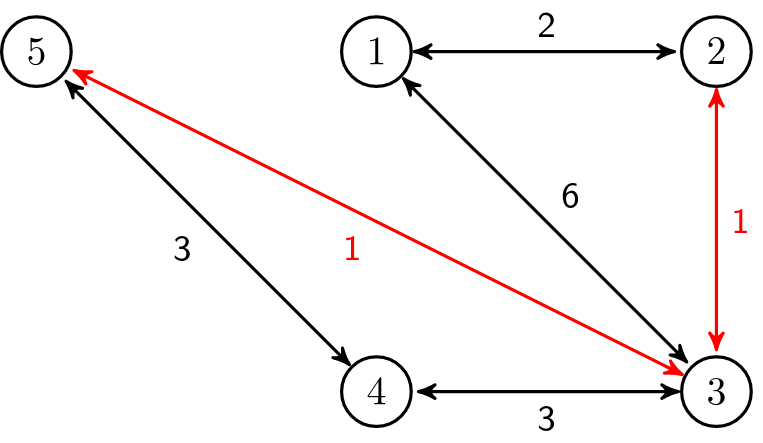
\includegraphics[scale=0.25]{imagenes/ejemplo1.png}
\end{minipage}

\bigskip

Entonces, tendríamos las siguientes respuestas para cada uno de los problemas planteados:

\begin{enumerate}
	\item Camino mínimo de 1 a 5 con 2 rutas premium: \textbf{4}

	\item Camino mínimo de 1 a 5 con 1 rutas premium: \textbf{7}
	
	\item Camino mínimo de 1 a 5 con 0 rutas premium: \textbf{12}
	
	\item Camino mínimo de 3 a 5 con 1 rutas premium: \textbf{1}
	
	\item Camino mínimo de 3 a 5 con 0 rutas premium: \textbf{6}
\end{enumerate}

\subsection{Desarrollo}
Dado este problema, podemos modelarlo utilizando grafos. Así, cada ciudad se representaría con un nodo, y cada una de las rutas que conecta dos ciudades, con una arista. Del mismo modo, el problema pasaría a ser alcanzar el camino mínimo de un nodo origen a un nodo destino, utilizando como máximo k aristas premium; y dado que las rutas son bidireccionales, podemos utilizar un grafo común no dirigido para esta representación.

A partir de esta representación, podemos poner el foco en las dificultades que trae consigo el problema. Sabemos que utilizando un algoritmo de camino mínimo, obtendríamos el camino más corto desde el nodo origen al nodo destino, pero nada sabríamos sobre cuantas rutas premium se están utilizando. De este modo, si bien tenemos una aproximación buena del problema, tenemos que buscar la manera de poner en consideración las rutas premium y su uso. 

Un buen punto de inicio es considerar que, si bien tenemos un límite de rutas premium, podríamos encontrar un mejor camino que utilice una menor cantidad. Por ende, no alcanza con encontrar el camino mínimo que utilice k rutas premium, sino que debemos encontrar el mínimo de todos aquellos que utilicen hasta k premium. Es decir que, en lugar de plantearlo como un único problema, podríamos ver el ejercicio como la mejor solución de k subproblemas distintos, donde el i-ésimo subproblema nos da el camino mínimo utilizando exactamente $i$ rutas premium.

Por otro lado, aún buscando resolver solo uno de los subproblemas planteados, estaríamos frente a la posibilidad de alcanzar el límite de rutas antes de recorrer todas (y por ende, de estar tomando una decisión errónea). Debemos, entonces, buscar la manera de llegar al último nodo habiendo elegido las mejores rutas premium posibles, siendo que no haya forma de tomar una ruta premium distinta y a través de ella se consiga un camino de menor distancia.

Para enfrentar este problema, podríamos generar un grafo con $k$ níveles, donde cada nivel sea una copia exacta del grafo original, y el nodo J perteneciente al i-ésimo nivel represente que para llegar a ese nodo se utilizaron $i$ rutas premium desde el nodo origen. De este modo, pasamos a tener un grafo de $nk$ nodos, donde cualquiera de los caminos entre el nodo origen y los k nodos destinos pueden representar una respuesta válida.

Sin embargo, modelando el grafo de esta manera tendríamos problemas, puesto que nuestro grafo inicial era no dirigido y nuestra idea es que cada nivel represente la cantidad de rutas premium utilizadas hasta el momento. Por ende, no podría ocurrir que se pase de un nodo perteneciente del nivel $i+1$ a un nodo del nivel $i$, ya que esto implicaría que, al utilizar una ruta premium más, disminuyó el nivel (es decir que disminuyó la cantidad de rutas premium utilizadas, siguiendo la idea de nuestro modelo, lo cual sería absurdo). Por lo tanto, debemos modelar el nuevo grafo de manera que:

\begin{enumerate}
	\item Debe haber un nivel por cada posible respuesta

	\item Cada vez que se utiliza una ruta premium, se sube de nivel

	\item Cada vez que se utiliza una ruta que no es premium, se mantiene el mismo nivel

	\item Se deben mantener las conexiones del grafo original (debe ser una representación fiel)
\end{enumerate}

Dadas estas condiciones, tendremos un grafo con $k$ niveles, como habíamos establecido anteriormente, pero debido a que hay rutas que solo se pueden recorrer en una dirección, tendremos que usar un \underline{\textbf{grafo dirigido}}. En él, estableceremos dos tipos de relaciones, que aplicarán para todos los niveles del grafo.

La primer relación a definir será entre los nodos conectados por una arista común. No es dificil ver que, si en el grafo original había una arista común entre el nodo J y el nodo H de peso $P$, ahora habrá $k$ representaciones de esa misma arista, para los nodos $J_i$ y $H_i$ con i entre 0 y k, donde el peso de cada una de ellas será $P$. Al ser nuestro nuevo grafo un digrafo, y como establecimos que cuando no se usa una ruta premium se mantiene el mismo nivel, bien podría ocurrir que nuestro camino vaya de $J_i$ a $H_i$ o viceversa, por lo que utilizaremos una arista para cada una de estas posibilidades. Es decir que, para cada nivel i, habrá una arista dirigida que conecte $J_i$ con $H_i$ y una que conecte $H_i$ con $J_i$. De este modo, quedan definidas de manera correcta todas las aristas no premium pertenecientes al grafo inicial.

La segunda relación a definir será entre los nodos conectados por una arista premium. Al igual que en el otro caso, por cada arista premium habrá $k$ representaciones de esta arista. Sin embargo, como al tomar una ruta premium debemos aumentar el nivel, hay que establecer una relación entre el i-ésimo y el (i+i)-ésimo nivel. Así, si en el grafo inicial había una arista premium entre los nodos J y K, ahora habrá una arista dirigida de $J_i$ a $K_i+1$ y una de $K_i$ a $J_i+1$. Notemos que, al tener una arista no dirigida en el grafo inicial, debe ser posible recorrer la ruta en ambas direcciones.

De esta manera, definimos nuestro grafo dirigido de $k$ niveles de manera que represente correctamente el grafo inicial y, por consecuente, a nuestro problema. Para dejar más en claro como se produce la creación del grafo, planteamos el siguiente algoritmo, donde consideramos que los ejes funcionan del mismo modo para grafos dirigidos y no dirigidos, y el grafo es el que distingue si una arista funciona de manera bidireccional o no; y que la estructura de eje es:

\begin{itemize}
	\item nat primerEje

	\item nat segundoEje

	\item nat peso
\end{itemize}

\begin{algorithm}[H]
	\NoCaptionOfAlgo
	\caption{\algoritmo{agregarEjeComun}{\In{e}{eje}, \In{n}{nat}, \In{k}{nat}, \Inout{grafoConNiveles}{digrafo}}{}}
	
	\For{c $\leq$ k}{
		nuevoPrimerNodo = e.primerNodo + c $\times$ n

		nuevoSegundoNodo = e.segundoNodo + c $\times$ n

		agregarEjeADigrafo(nuevoPrimerNodo, nuevoSegundoNodo, e.peso, grafoConNiveles)

		agregarEjeADigrafo(nuevoSegundoNodo, nuevoPrimerNodo, e.peso, grafoConNiveles)
	}
\end{algorithm}
	
\begin{algorithm}[H]
	\NoCaptionOfAlgo
	\caption{\algoritmo{agregarEjePremium}{\In{e}{eje}, \In{n}{nat}, \In{k}{nat}, \Inout{grafoConNiveles}{digrafo}}{}}
	
	\For{c $<$ k}{
		nuevoPrimerNodo = e.primerNodo + c $\times$ n

		nuevoSegundoNodo = e.segundoNodo + c $\times$ n

		agregarEjeADigrafo(nuevoPrimerNodo, (nuevoSegundoNodo + n), e.peso, grafoConNiveles)

		agregarEjeADigrafo(nuevoSegundoNodo, (nuevoPrimerNodo + n), e.peso, grafoConNiveles)
	}
\end{algorithm}

Con esta nueva representación, tendríamos un grafo similar al que se ve en imágen, donde el número que representa a cada nodo se define como:

\begin{center}
	$J_i =	J + c \times n$
\end{center}

siendo $J_i$ el número del nodo a agregar, $J$ el valor del nodo original, $c$ el nivel actual y $n$ la cantidad de nodos en el grafo. Es así que, $H$ y $F$ representan al mismo nodo $\Leftrightarrow$ $H$ $\equiv$ $F$ (mod $n$).

\smallskip

\noindent
\begin{minipage}{0.2\textwidth}
	\begin{center}
		\underline{\textbf{Grafo original}}
		\newline

		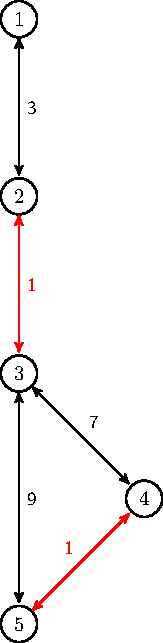
\includegraphics[scale=0.6]{imagenes/ej1_ex.pdf}
	\end{center}
\end{minipage}
\hfill
\begin{minipage}{0.3\textwidth}
	\begin{center}
		\underline{\textbf{Con K = 1}}
		\newline

		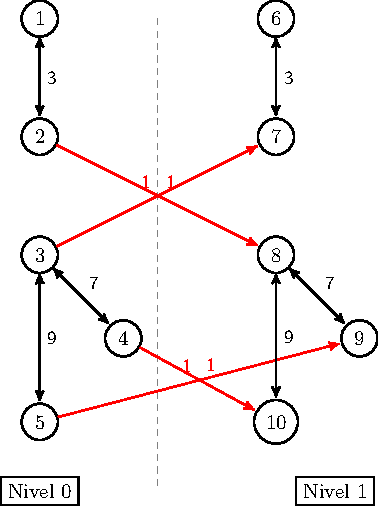
\includegraphics[scale=0.75]{imagenes/ej1_ex_k1.pdf}
	\end{center}
\end{minipage}
\hfill
\begin{minipage}{0.45\textwidth}
	\begin{center}
		\underline{\textbf{Con K = 2}}
		\newline

		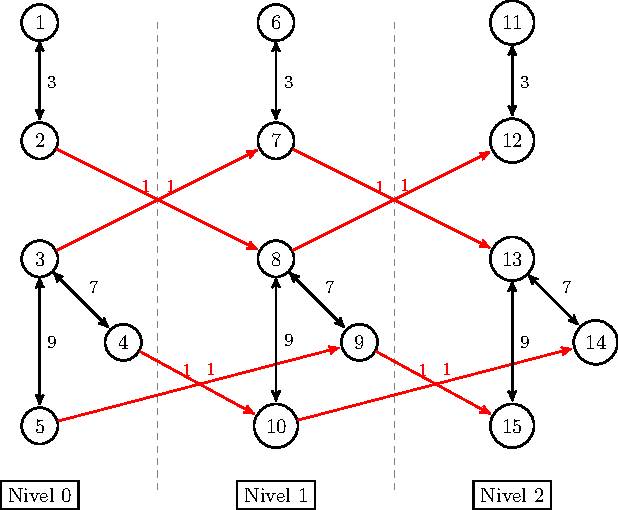
\includegraphics[scale=0.75]{imagenes/ej1_ex_k2.pdf}
	\end{center}
\end{minipage}

\smallskip

Dado que ya tenemos un grafo que nos permite identificar la cantidad de rutas premium utilizadas por la manera en la que está caracterizada cada nodo, basta con conocer nuestro nodo origen y buscar el camino más corto hasta las $k$ posibles soluciones, para luego quedarnos con la mejor solución.

Por lo tanto, como sabemos que el nodo origen necesariamente estará situado en el primer nivel (es decir, que es único para nuestros propósitos), podemos utilizar un algoritmo que nos de el camino mínimo de un nodo a todos los demás y luego evaluar solo aquellos que nos den una respuesta válida a nuestro problema (un camino de origen a destino).

En consecuencia, podríamos usar tanto el algoritmo de Bellman-Ford como el de Dijkstra. Sin embargo, considerando que no tenemos aristas con pesos negativos, y que el uso de Dijkstra nos facilita el cumplimiento dela complejidad, nos quedaremos con este algoritmo para realizar la búsqueda.

Por lo tanto, con lo visto anteriormente, acabaríamos teniendo un algoritmo de este estilo:

\begin{algorithm}[H]
	\NoCaptionOfAlgo
	\caption{\algoritmo{deliveryOptimo}{\In{origen}{nat}, \In{destino}{nat}, \In{n}{nat}, \In{k}{nat}, \In{ejesComunes}{lista[ejes]}, \In{ejesPremium}{lista[ejes]}}{nat}}	
	digrafo: grafoConNiveles $\leftarrow$ crearDigrafoVacio
	
	\For{e $\in$ ejesComunes}{
		agregarEjeComun(e, n, k, grafoConNiveles)
	}
	\For{e $\in$ ejesPremium}{
		agregarEjePremium(e, n, k, grafoConNiveles)
	}

	vector[nat]: distancias $\leftarrow$ dijkstra(grafoConNiveles, origen)
	
	\For{i $\leq$ k}{
		\If{distancias[destino + i $\times$ n] $<$ res}{
			res $\leftarrow$ distancias[destino + i $\times$ n]	
		}
	}
\end{algorithm}

\subsection{Cota temporal}
La cota temporal de este problema se puede reducir, como vemos en el algoritmo de deliveryOptimo que aparece en la sección \textbf{Desarrollo}, a conocer las complejidades de tres algoritmos:
\begin{itemize}
	\item agregarEjeComun

	\item agregarEjePremium
	
	\item Dijkstra
\end{itemize}

Veamos cual es la complejidad de cada uno de ellos:

\begin{center}
	\textbf{agregarEjeComun}
\end{center}

Este algoritmo toma un eje, un valor $n$ y un valor $k$, y agrega el mismo eje para cada uno de los niveles desde 0 a k. Por lo tanto, como agregar un eje se compone de tres asignaciones de costo $O(1)$, el costo del algoritmo se reduce al $for$ que se encarga de realizar la misma acción para todos los niveles. Por lo tanto, su costo es $O(k)$, donde k representa el límite de rutas premium que se puede utilizar.

\begin{center}
	\textbf{agregarEjePremium}
\end{center}

Este algoritmo realiza las mismas acciones que $agregarEjeComun$, pero reasigna los ejes de manera distinta. Sin embargo, como aún realiza asignaciones de costo $O(1)$, podemos reducir la complejidad otra vez al ciclo que posee. Por lo tanto, como vimos con el algoritmo anterior, el costo es $O(k)$, donde k representa el límite de rutas premium que se puede utilizar.

\begin{center}
	\textbf{Dijkstra}
\end{center}

El algoritmo de Dijkstra. Al usar la implementación y las estructuras que vimos en clase, obtenemos un costo de $O(n^2)$, donde n es la cantidad de nodos del grafo que recibimos en la entrada.\bigskip

Ahora, queda ver como nos afectan estas complejidades al algoritmo de deliveryOptimo. En este algoritmo, usamos dos ciclos: uno para los ejes comunes, y uno para los ejes premium. Como sabemos que la cantidad total de ejes es $m$, y que el costo de agregarEjePremium y de agregarEjeComun es $O(k)$, al aplicarle uno de estos dos algoritmos a todos los ejes tenemos una complejidad de $O(mk)$.

Luego, generamos el vector de distancias aplicandole Dijkstra al grafo con $k+1$ niveles que generamos. Sin embargo, como nuestro grafo tiene $k+1$ repeticiones del grafo inicial, acaba teniendo $k$ veces $n$ nodos; es decir, $nk$ nodos en total. Por lo tanto, al aplicarle Dijkstra, como la complejidad depende de la cantidad de nodos en el grafo, tendrá un costo de $O((n(k+1))^2)$, que se puede acotar por $O((nk)^2)$

Finalmente, recorremos todos los niveles para buscar el camino mínimo que va de origen a destino y utiliza entre 0 y k rutas premium. Esto implica un último ciclo, donde se recorren las $k$ posibles soluciones, lo que nos da un costo de $O(k)$.

En resumen, tenemos tres costos significativos en nuestro algoritmo:

\begin{itemize}
	\item $O(mk)$

	\item $O((nk)^2)$

	\item $O(k)$
\end{itemize}

Es trivial notar que $O(k)$ $\subseteq$ $O(mk)$, por lo que $O(k)$ + $O(mk)$ $\subseteq$ $O(k + mk)$ $\subseteq$ $O(m(k+1)$ $\subseteq$ $O(mk)$. Por otra parte, por propiedades de arbol, sabemos que m $\leq$ $n^2$ para cualquier grafo; por lo tanto, podemos acotar $m$ por $n^2$. Entonces, $O(m)$ $\subseteq$ $O(n^2)$ $\rightarrow$ $O(mk)$ $\subseteq$ $O(kn^2)$ $\subseteq$ $O((nk)^2)$. Por lo tanto, $O(mk + (nk)^2)$ $\subseteq$ $O((nk)^2)$.

Por lo visto en el parrafo anterior, tenemos: $O(mk + k + (nk)^2)$ $\subseteq$ $O((nk)^2)$. Por lo tanto, nuestro algoritmo tiene complejidad $O((nk)^2)$ que es igual a $O(n^2k^2)$.

\subsection{Experimentacion}

De cara a la experimentación, nuestra expectativa es que la performance del algoritmo se vea afectada por dos factores: la cantidad de ciudades (n) y la cantidad máxima de rutas premium a utilizar (k). Consideramos que la cantidad de rutas (m) no debería afectar los tiempos por la representación interna escogida al correr Dijkstra (matriz de adyacencia). Por un motivo similar, asumimos que la cantidad de rutas premium existentes tampoco debería influir en el timepo de ejecución, ya que es k quien determina la cantidad de niveles del supergrafo.

La metodología de prueba y medición de tiempo se encuentra detallada en los apéndices. Los siguientes gráficos corresponden a cada una de las variables aisladas, manteniendo todas las otras fijas en un mismo numero en tanto esto es posible.

\begin{center}
	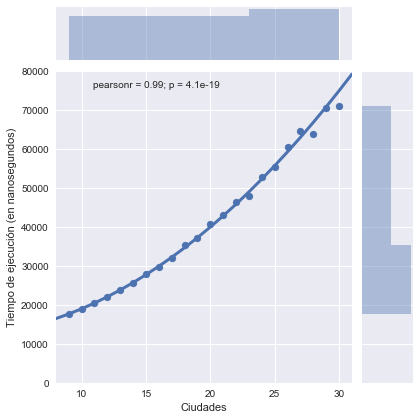
\includegraphics[scale=0.5]{imagenes/ej1-1.png}
\end{center}

Como se puede apreciar en este gráfico, el tiempo de ejecución depende fuertemente la cantidad de ciudades. Esto no es una sorpresa, ya que como hemos mencionado nuestra cota de complejidad es $O(n^2k^2)$.

\begin{center}
	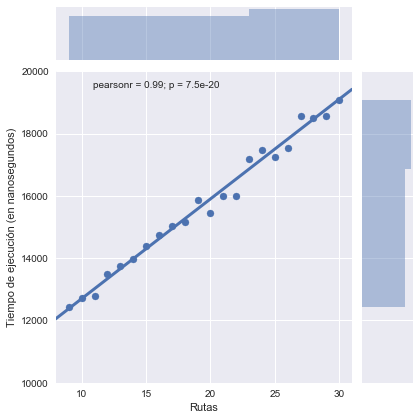
\includegraphics[scale=0.5]{imagenes/ej1-2.png}
\end{center}

En este gráfico, podemos notar que si bien la cantidad de rutas no define la complejidad del algoritmo (hay otros aspectos que definen la complejidad), en nuestra implementación tienen un impacto lineal. Esto se condice con el costo $O(mk)$ previamente mencionado.

\begin{center}
	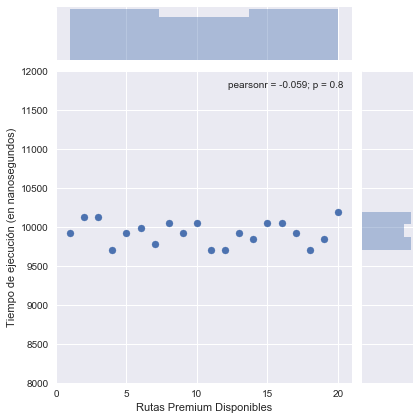
\includegraphics[scale=0.5]{imagenes/ej1-3.png}
\end{center}

Como esperábamos, la cantidad de rutas premium totales no influye en la complejidad si no modificamos la cantidad total de rutas o los niveles del supergrafo.

\begin{center}
	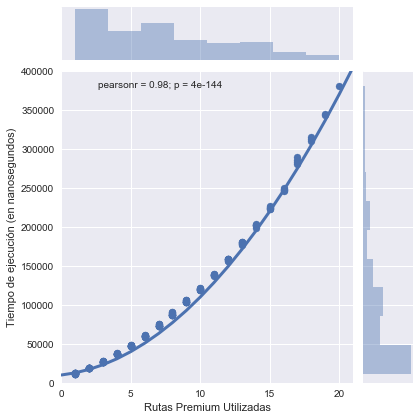
\includegraphics[scale=0.5]{imagenes/ej1-4.png}
\end{center}

Por otro lado, al aumentar la cantidad máxima de rutas premium utilizables, el impacto es nuevamente cuadrático. También se puede ver que la correlación entre tiempo de ejecución y k es más fuerte, ya que los 3 costos mencionados dependen de k.

A su vez, en este gráfico no se limitó el total de rutas premium existentes, y se puede ver nuevamente que dicho valor no influye en la complejidad.
